% Graphic for TeX using PGF
% Title: /home/jcelerier/travail/rapport-audio-iscore/images/unity-1.dia
% Creator: Dia v0.97+git
% CreationDate: Tue Feb  9 12:32:28 2016
% For: jcelerier
% \usepackage{tikz}
% The following commands are not supported in PSTricks at present
% We define them conditionally, so when they are implemented,
% this pgf file will use them.
\ifx\du\undefined
  \newlength{\du}
\fi
\setlength{\du}{15\unitlength}
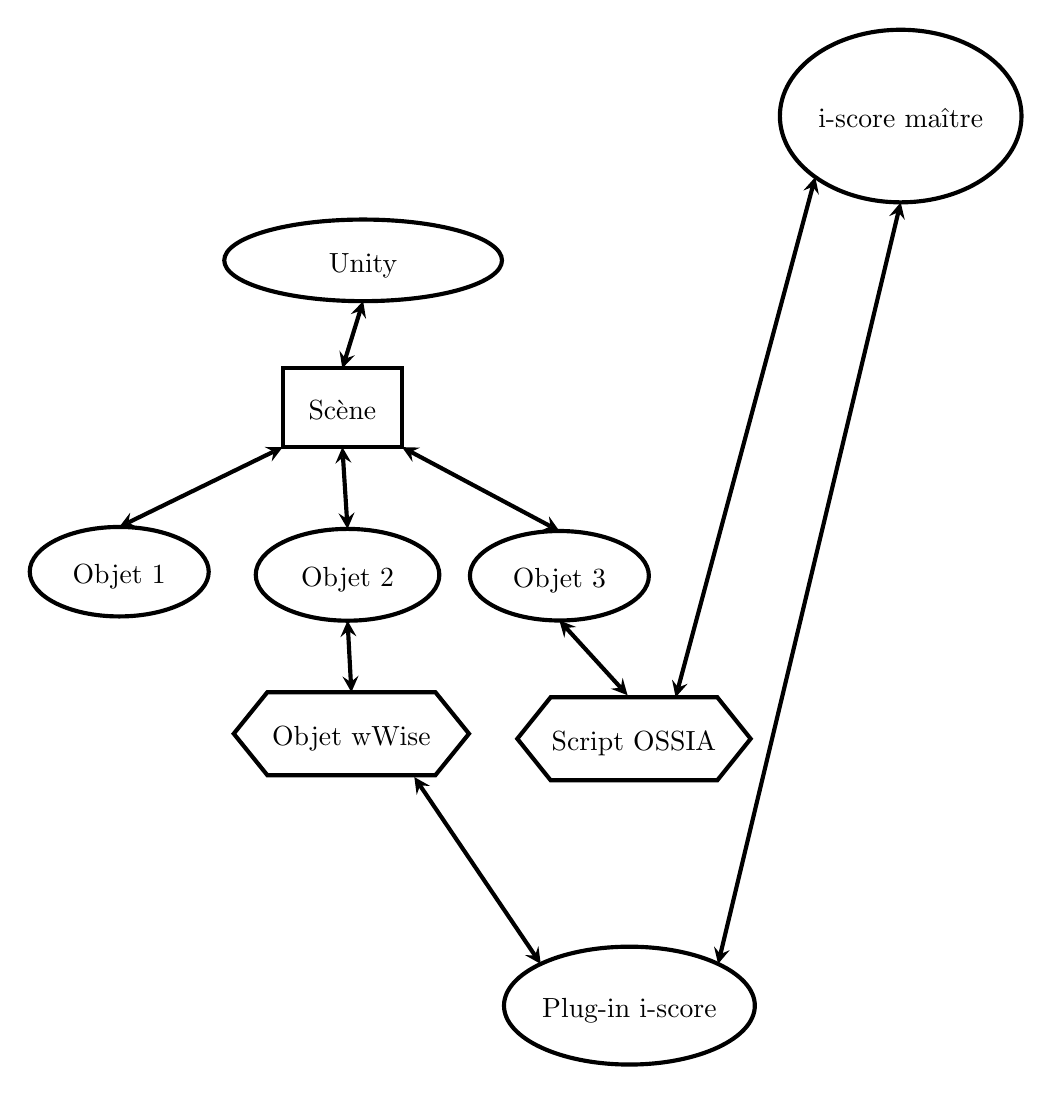
\begin{tikzpicture}[even odd rule]
\pgftransformxscale{1.000000}
\pgftransformyscale{-1.000000}
\definecolor{dialinecolor}{rgb}{0.000000, 0.000000, 0.000000}
\pgfsetstrokecolor{dialinecolor}
\pgfsetstrokeopacity{1.000000}
\definecolor{diafillcolor}{rgb}{1.000000, 1.000000, 1.000000}
\pgfsetfillcolor{diafillcolor}
\pgfsetfillopacity{1.000000}
\pgfsetlinewidth{0.100000\du}
\pgfsetdash{}{0pt}
\pgfsetmiterjoin
\definecolor{diafillcolor}{rgb}{1.000000, 1.000000, 1.000000}
\pgfsetfillcolor{diafillcolor}
\pgfsetfillopacity{1.000000}
\pgfpathellipse{\pgfpoint{40.058431\du}{14.165916\du}}{\pgfpoint{2.910031\du}{0\du}}{\pgfpoint{0\du}{2.078716\du}}
\pgfusepath{fill}
\definecolor{dialinecolor}{rgb}{0.000000, 0.000000, 0.000000}
\pgfsetstrokecolor{dialinecolor}
\pgfsetstrokeopacity{1.000000}
\pgfpathellipse{\pgfpoint{40.058431\du}{14.165916\du}}{\pgfpoint{2.910031\du}{0\du}}{\pgfpoint{0\du}{2.078716\du}}
\pgfusepath{stroke}
% setfont left to latex
\definecolor{dialinecolor}{rgb}{0.000000, 0.000000, 0.000000}
\pgfsetstrokecolor{dialinecolor}
\pgfsetstrokeopacity{1.000000}
\definecolor{diafillcolor}{rgb}{0.000000, 0.000000, 0.000000}
\pgfsetfillcolor{diafillcolor}
\pgfsetfillopacity{1.000000}
\node[anchor=base,inner sep=0pt, outer sep=0pt,color=dialinecolor] at (40.058431\du,14.450916\du){i-score maître};
\pgfsetlinewidth{0.100000\du}
\pgfsetdash{}{0pt}
\pgfsetmiterjoin
\definecolor{diafillcolor}{rgb}{1.000000, 1.000000, 1.000000}
\pgfsetfillcolor{diafillcolor}
\pgfsetfillopacity{1.000000}
\pgfpathellipse{\pgfpoint{27.108448\du}{17.642281\du}}{\pgfpoint{3.345148\du}{0\du}}{\pgfpoint{0\du}{0.982881\du}}
\pgfusepath{fill}
\definecolor{dialinecolor}{rgb}{0.000000, 0.000000, 0.000000}
\pgfsetstrokecolor{dialinecolor}
\pgfsetstrokeopacity{1.000000}
\pgfpathellipse{\pgfpoint{27.108448\du}{17.642281\du}}{\pgfpoint{3.345148\du}{0\du}}{\pgfpoint{0\du}{0.982881\du}}
\pgfusepath{stroke}
% setfont left to latex
\definecolor{dialinecolor}{rgb}{0.000000, 0.000000, 0.000000}
\pgfsetstrokecolor{dialinecolor}
\pgfsetstrokeopacity{1.000000}
\definecolor{diafillcolor}{rgb}{0.000000, 0.000000, 0.000000}
\pgfsetfillcolor{diafillcolor}
\pgfsetfillopacity{1.000000}
\node[anchor=base,inner sep=0pt, outer sep=0pt,color=dialinecolor] at (27.108448\du,17.927281\du){Unity};
\pgfsetlinewidth{0.100000\du}
\pgfsetdash{}{0pt}
\pgfsetmiterjoin
{\pgfsetcornersarced{\pgfpoint{0.000000\du}{0.000000\du}}\definecolor{diafillcolor}{rgb}{1.000000, 1.000000, 1.000000}
\pgfsetfillcolor{diafillcolor}
\pgfsetfillopacity{1.000000}
\fill (25.171000\du,20.242200\du)--(25.171000\du,22.142200\du)--(28.046000\du,22.142200\du)--(28.046000\du,20.242200\du)--cycle;
}{\pgfsetcornersarced{\pgfpoint{0.000000\du}{0.000000\du}}\definecolor{dialinecolor}{rgb}{0.000000, 0.000000, 0.000000}
\pgfsetstrokecolor{dialinecolor}
\pgfsetstrokeopacity{1.000000}
\draw (25.171000\du,20.242200\du)--(25.171000\du,22.142200\du)--(28.046000\du,22.142200\du)--(28.046000\du,20.242200\du)--cycle;
}% setfont left to latex
\definecolor{dialinecolor}{rgb}{0.000000, 0.000000, 0.000000}
\pgfsetstrokecolor{dialinecolor}
\pgfsetstrokeopacity{1.000000}
\definecolor{diafillcolor}{rgb}{0.000000, 0.000000, 0.000000}
\pgfsetfillcolor{diafillcolor}
\pgfsetfillopacity{1.000000}
\node[anchor=base,inner sep=0pt, outer sep=0pt,color=dialinecolor] at (26.608500\du,21.477200\du){Scène};
\pgfsetlinewidth{0.100000\du}
\pgfsetdash{}{0pt}
\pgfsetmiterjoin
\definecolor{diafillcolor}{rgb}{1.000000, 1.000000, 1.000000}
\pgfsetfillcolor{diafillcolor}
\pgfsetfillopacity{1.000000}
\pgfpathellipse{\pgfpoint{21.233458\du}{25.142229\du}}{\pgfpoint{2.155658\du}{0\du}}{\pgfpoint{0\du}{1.077829\du}}
\pgfusepath{fill}
\definecolor{dialinecolor}{rgb}{0.000000, 0.000000, 0.000000}
\pgfsetstrokecolor{dialinecolor}
\pgfsetstrokeopacity{1.000000}
\pgfpathellipse{\pgfpoint{21.233458\du}{25.142229\du}}{\pgfpoint{2.155658\du}{0\du}}{\pgfpoint{0\du}{1.077829\du}}
\pgfusepath{stroke}
% setfont left to latex
\definecolor{dialinecolor}{rgb}{0.000000, 0.000000, 0.000000}
\pgfsetstrokecolor{dialinecolor}
\pgfsetstrokeopacity{1.000000}
\definecolor{diafillcolor}{rgb}{0.000000, 0.000000, 0.000000}
\pgfsetfillcolor{diafillcolor}
\pgfsetfillopacity{1.000000}
\node[anchor=base,inner sep=0pt, outer sep=0pt,color=dialinecolor] at (21.233458\du,25.427229\du){Objet 1};
\pgfsetlinewidth{0.100000\du}
\pgfsetdash{}{0pt}
\pgfsetmiterjoin
\definecolor{diafillcolor}{rgb}{1.000000, 1.000000, 1.000000}
\pgfsetfillcolor{diafillcolor}
\pgfsetfillopacity{1.000000}
\pgfpathellipse{\pgfpoint{26.733491\du}{25.217196\du}}{\pgfpoint{2.211191\du}{0\du}}{\pgfpoint{0\du}{1.105596\du}}
\pgfusepath{fill}
\definecolor{dialinecolor}{rgb}{0.000000, 0.000000, 0.000000}
\pgfsetstrokecolor{dialinecolor}
\pgfsetstrokeopacity{1.000000}
\pgfpathellipse{\pgfpoint{26.733491\du}{25.217196\du}}{\pgfpoint{2.211191\du}{0\du}}{\pgfpoint{0\du}{1.105596\du}}
\pgfusepath{stroke}
% setfont left to latex
\definecolor{dialinecolor}{rgb}{0.000000, 0.000000, 0.000000}
\pgfsetstrokecolor{dialinecolor}
\pgfsetstrokeopacity{1.000000}
\definecolor{diafillcolor}{rgb}{0.000000, 0.000000, 0.000000}
\pgfsetfillcolor{diafillcolor}
\pgfsetfillopacity{1.000000}
\node[anchor=base,inner sep=0pt, outer sep=0pt,color=dialinecolor] at (26.733491\du,25.502196\du){Objet 2 };
\pgfsetlinewidth{0.100000\du}
\pgfsetdash{}{0pt}
\pgfsetbuttcap
\pgfsetmiterjoin
\pgfsetlinewidth{0.100000\du}
\pgfsetbuttcap
\pgfsetmiterjoin
\pgfsetdash{}{0pt}
\definecolor{diafillcolor}{rgb}{1.000000, 1.000000, 1.000000}
\pgfsetfillcolor{diafillcolor}
\pgfsetfillopacity{1.000000}
\definecolor{dialinecolor}{rgb}{0.000000, 0.000000, 0.000000}
\pgfsetstrokecolor{dialinecolor}
\pgfsetstrokeopacity{1.000000}
\pgfpathmoveto{\pgfpoint{31.625900\du}{28.167200\du}}
\pgfpathlineto{\pgfpoint{35.640900\du}{28.167200\du}}
\pgfpathlineto{\pgfpoint{36.443900\du}{29.167200\du}}
\pgfpathlineto{\pgfpoint{35.640900\du}{30.167200\du}}
\pgfpathlineto{\pgfpoint{31.625900\du}{30.167200\du}}
\pgfpathlineto{\pgfpoint{30.822900\du}{29.167200\du}}
\pgfpathlineto{\pgfpoint{31.625900\du}{28.167200\du}}
\pgfpathclose
\pgfusepath{fill,stroke}
% setfont left to latex
\definecolor{dialinecolor}{rgb}{0.000000, 0.000000, 0.000000}
\pgfsetstrokecolor{dialinecolor}
\pgfsetstrokeopacity{1.000000}
\definecolor{diafillcolor}{rgb}{0.000000, 0.000000, 0.000000}
\pgfsetfillcolor{diafillcolor}
\pgfsetfillopacity{1.000000}
\node[anchor=base,inner sep=0pt, outer sep=0pt,color=dialinecolor] at (33.633400\du,29.447200\du){Script OSSIA};
\pgfsetlinewidth{0.100000\du}
\pgfsetdash{}{0pt}
\pgfsetmiterjoin
\definecolor{diafillcolor}{rgb}{1.000000, 1.000000, 1.000000}
\pgfsetfillcolor{diafillcolor}
\pgfsetfillopacity{1.000000}
\pgfpathellipse{\pgfpoint{31.836558\du}{25.240029\du}}{\pgfpoint{2.155658\du}{0\du}}{\pgfpoint{0\du}{1.077829\du}}
\pgfusepath{fill}
\definecolor{dialinecolor}{rgb}{0.000000, 0.000000, 0.000000}
\pgfsetstrokecolor{dialinecolor}
\pgfsetstrokeopacity{1.000000}
\pgfpathellipse{\pgfpoint{31.836558\du}{25.240029\du}}{\pgfpoint{2.155658\du}{0\du}}{\pgfpoint{0\du}{1.077829\du}}
\pgfusepath{stroke}
% setfont left to latex
\definecolor{dialinecolor}{rgb}{0.000000, 0.000000, 0.000000}
\pgfsetstrokecolor{dialinecolor}
\pgfsetstrokeopacity{1.000000}
\definecolor{diafillcolor}{rgb}{0.000000, 0.000000, 0.000000}
\pgfsetfillcolor{diafillcolor}
\pgfsetfillopacity{1.000000}
\node[anchor=base,inner sep=0pt, outer sep=0pt,color=dialinecolor] at (31.836558\du,25.525029\du){Objet 3};
\pgfsetlinewidth{0.100000\du}
\pgfsetdash{}{0pt}
\pgfsetbuttcap
{
\definecolor{diafillcolor}{rgb}{0.000000, 0.000000, 0.000000}
\pgfsetfillcolor{diafillcolor}
\pgfsetfillopacity{1.000000}
% was here!!!
\pgfsetarrowsstart{stealth}
\pgfsetarrowsend{stealth}
\definecolor{dialinecolor}{rgb}{0.000000, 0.000000, 0.000000}
\pgfsetstrokecolor{dialinecolor}
\pgfsetstrokeopacity{1.000000}
\draw (27.108400\du,18.625100\du)--(26.608500\du,20.242200\du);
}
\pgfsetlinewidth{0.100000\du}
\pgfsetdash{}{0pt}
\pgfsetbuttcap
{
\definecolor{diafillcolor}{rgb}{0.000000, 0.000000, 0.000000}
\pgfsetfillcolor{diafillcolor}
\pgfsetfillopacity{1.000000}
% was here!!!
\pgfsetarrowsstart{stealth}
\pgfsetarrowsend{stealth}
\definecolor{dialinecolor}{rgb}{0.000000, 0.000000, 0.000000}
\pgfsetstrokecolor{dialinecolor}
\pgfsetstrokeopacity{1.000000}
\draw (25.171000\du,22.142200\du)--(21.233500\du,24.064400\du);
}
\pgfsetlinewidth{0.100000\du}
\pgfsetdash{}{0pt}
\pgfsetbuttcap
{
\definecolor{diafillcolor}{rgb}{0.000000, 0.000000, 0.000000}
\pgfsetfillcolor{diafillcolor}
\pgfsetfillopacity{1.000000}
% was here!!!
\pgfsetarrowsstart{stealth}
\pgfsetarrowsend{stealth}
\definecolor{dialinecolor}{rgb}{0.000000, 0.000000, 0.000000}
\pgfsetstrokecolor{dialinecolor}
\pgfsetstrokeopacity{1.000000}
\draw (26.608500\du,22.142200\du)--(26.733500\du,24.111600\du);
}
\pgfsetlinewidth{0.100000\du}
\pgfsetdash{}{0pt}
\pgfsetbuttcap
{
\definecolor{diafillcolor}{rgb}{0.000000, 0.000000, 0.000000}
\pgfsetfillcolor{diafillcolor}
\pgfsetfillopacity{1.000000}
% was here!!!
\pgfsetarrowsstart{stealth}
\pgfsetarrowsend{stealth}
\definecolor{dialinecolor}{rgb}{0.000000, 0.000000, 0.000000}
\pgfsetstrokecolor{dialinecolor}
\pgfsetstrokeopacity{1.000000}
\draw (28.046000\du,22.142200\du)--(31.836600\du,24.162200\du);
}
\pgfsetlinewidth{0.100000\du}
\pgfsetdash{}{0pt}
\pgfsetbuttcap
{
\definecolor{diafillcolor}{rgb}{0.000000, 0.000000, 0.000000}
\pgfsetfillcolor{diafillcolor}
\pgfsetfillopacity{1.000000}
% was here!!!
\pgfsetarrowsstart{stealth}
\pgfsetarrowsend{stealth}
\definecolor{dialinecolor}{rgb}{0.000000, 0.000000, 0.000000}
\pgfsetstrokecolor{dialinecolor}
\pgfsetstrokeopacity{1.000000}
\draw (31.836600\du,26.317900\du)--(33.478612\du,28.117495\du);
}
\pgfsetlinewidth{0.100000\du}
\pgfsetdash{}{0pt}
\pgfsetbuttcap
{
\definecolor{diafillcolor}{rgb}{0.000000, 0.000000, 0.000000}
\pgfsetfillcolor{diafillcolor}
\pgfsetfillopacity{1.000000}
% was here!!!
\pgfsetarrowsstart{stealth}
\pgfsetarrowsend{stealth}
\definecolor{dialinecolor}{rgb}{0.000000, 0.000000, 0.000000}
\pgfsetstrokecolor{dialinecolor}
\pgfsetstrokeopacity{1.000000}
\draw (38.000700\du,15.635800\du)--(34.637200\du,28.167200\du);
}
\pgfsetlinewidth{0.100000\du}
\pgfsetdash{}{0pt}
\pgfsetmiterjoin
\definecolor{diafillcolor}{rgb}{1.000000, 1.000000, 1.000000}
\pgfsetfillcolor{diafillcolor}
\pgfsetfillopacity{1.000000}
\pgfpathellipse{\pgfpoint{33.523394\du}{35.595349\du}}{\pgfpoint{3.021094\du}{0\du}}{\pgfpoint{0\du}{1.419749\du}}
\pgfusepath{fill}
\definecolor{dialinecolor}{rgb}{0.000000, 0.000000, 0.000000}
\pgfsetstrokecolor{dialinecolor}
\pgfsetstrokeopacity{1.000000}
\pgfpathellipse{\pgfpoint{33.523394\du}{35.595349\du}}{\pgfpoint{3.021094\du}{0\du}}{\pgfpoint{0\du}{1.419749\du}}
\pgfusepath{stroke}
% setfont left to latex
\definecolor{dialinecolor}{rgb}{0.000000, 0.000000, 0.000000}
\pgfsetstrokecolor{dialinecolor}
\pgfsetstrokeopacity{1.000000}
\definecolor{diafillcolor}{rgb}{0.000000, 0.000000, 0.000000}
\pgfsetfillcolor{diafillcolor}
\pgfsetfillopacity{1.000000}
\node[anchor=base,inner sep=0pt, outer sep=0pt,color=dialinecolor] at (33.523394\du,35.880349\du){Plug-in i-score};
\pgfsetlinewidth{0.100000\du}
\pgfsetdash{}{0pt}
\pgfsetbuttcap
\pgfsetmiterjoin
\pgfsetlinewidth{0.100000\du}
\pgfsetbuttcap
\pgfsetmiterjoin
\pgfsetdash{}{0pt}
\definecolor{diafillcolor}{rgb}{1.000000, 1.000000, 1.000000}
\pgfsetfillcolor{diafillcolor}
\pgfsetfillopacity{1.000000}
\definecolor{dialinecolor}{rgb}{0.000000, 0.000000, 0.000000}
\pgfsetstrokecolor{dialinecolor}
\pgfsetstrokeopacity{1.000000}
\pgfpathmoveto{\pgfpoint{24.801700\du}{28.044700\du}}
\pgfpathlineto{\pgfpoint{28.849200\du}{28.044700\du}}
\pgfpathlineto{\pgfpoint{29.658700\du}{29.044700\du}}
\pgfpathlineto{\pgfpoint{28.849200\du}{30.044700\du}}
\pgfpathlineto{\pgfpoint{24.801700\du}{30.044700\du}}
\pgfpathlineto{\pgfpoint{23.992200\du}{29.044700\du}}
\pgfpathlineto{\pgfpoint{24.801700\du}{28.044700\du}}
\pgfpathclose
\pgfusepath{fill,stroke}
% setfont left to latex
\definecolor{dialinecolor}{rgb}{0.000000, 0.000000, 0.000000}
\pgfsetstrokecolor{dialinecolor}
\pgfsetstrokeopacity{1.000000}
\definecolor{diafillcolor}{rgb}{0.000000, 0.000000, 0.000000}
\pgfsetfillcolor{diafillcolor}
\pgfsetfillopacity{1.000000}
\node[anchor=base,inner sep=0pt, outer sep=0pt,color=dialinecolor] at (26.825450\du,29.324700\du){Objet wWise};
\pgfsetlinewidth{0.100000\du}
\pgfsetdash{}{0pt}
\pgfsetbuttcap
{
\definecolor{diafillcolor}{rgb}{0.000000, 0.000000, 0.000000}
\pgfsetfillcolor{diafillcolor}
\pgfsetfillopacity{1.000000}
% was here!!!
\pgfsetarrowsstart{stealth}
\pgfsetarrowsend{stealth}
\definecolor{dialinecolor}{rgb}{0.000000, 0.000000, 0.000000}
\pgfsetstrokecolor{dialinecolor}
\pgfsetstrokeopacity{1.000000}
\draw (26.733500\du,26.322800\du)--(26.825500\du,28.044700\du);
}
\pgfsetlinewidth{0.100000\du}
\pgfsetdash{}{0pt}
\pgfsetbuttcap
{
\definecolor{diafillcolor}{rgb}{0.000000, 0.000000, 0.000000}
\pgfsetfillcolor{diafillcolor}
\pgfsetfillopacity{1.000000}
% was here!!!
\pgfsetarrowsstart{stealth}
\pgfsetarrowsend{stealth}
\definecolor{dialinecolor}{rgb}{0.000000, 0.000000, 0.000000}
\pgfsetstrokecolor{dialinecolor}
\pgfsetstrokeopacity{1.000000}
\draw (28.342161\du,30.090123\du)--(31.387200\du,34.591400\du);
}
\pgfsetlinewidth{0.100000\du}
\pgfsetdash{}{0pt}
\pgfsetbuttcap
{
\definecolor{diafillcolor}{rgb}{0.000000, 0.000000, 0.000000}
\pgfsetfillcolor{diafillcolor}
\pgfsetfillopacity{1.000000}
% was here!!!
\pgfsetarrowsstart{stealth}
\pgfsetarrowsend{stealth}
\definecolor{dialinecolor}{rgb}{0.000000, 0.000000, 0.000000}
\pgfsetstrokecolor{dialinecolor}
\pgfsetstrokeopacity{1.000000}
\draw (40.058400\du,16.244700\du)--(35.659600\du,34.591400\du);
}
\end{tikzpicture}
